\chapter{L'oscillateur de Duffing forcé}
%
Considérons de nouveau un oscillateur forcé, mais maintenant avec un terme en $x^3$ supplémentaire, nous donnant l'équation de Duffing forcé. Ce n'est plus une équation linéaire, donc on ne peut plus exprimer la solution comme étant une superposition des solutions homogènes et particulières. Cette équation, comme la plupart des équations différentielles non-linéaires, n'a pas de solution analytique exacte.
%
%Limite faible de $\epsilon$
%
\begin{equation}
    \ddot{x} + \omega_0^2 x + \epsilon \gamma \dot{x} + \epsilon x^3 = \epsilon f_0 \cos(\omega t)
    \label{eq:duffing}
\end{equation}
%DO $f_0 \to \epsilon f_0$ CHANGE
%
%Aussi faible qu'il soit, ce terme invalide principe de superposition. Mais on peut faire des hypothèses a partir de faible amplitude...
%Lorsque $0 < \epsilon \ll 1$, on s'attend à trouver un comportement semblable à l'oscillateur harmonique forcé. 
%On cherche donc des solutions de la forme :
%on peut traiter le système comme étant un oscillateur harmonique perturbé. 
%En s'inspirant de l'oscillateur harmonique forcé, 
%On fait l'hypothèse que comme dans le cas de l'oscillateur harmonique amorti, la vitesse d'évolution de $r$ et de $\phi$ sont données par le coefficient d'amortissement $\gamma$. 
%Donc si $\gamma \ll \omega$,  $r$ et $\phi$ vont varier
% lentement par rapport à la période d'oscillation de $x$.
%nous allons employer une méthode d'analyse approximative appelée 
\section{La méthode de moyennement}
%
Afin d'analyser ce problème, nous allons utiliser la méthode de 
moyennement \cite{rand_lecture_2012} - un algorithme %développé dans les années 1930 par Krylov et %Bogoliubov pour 
qui nous permet de chercher des solutions approximatives à des équations de la forme :
\begin{equation}
    \ddot{x} + \omega_0^2 x = \epsilon g(x, \dot{x}, t)
\end{equation}
Où $\epsilon$ est un petit paramètre et $g$ est une fonction non-linéaire. Pour notre problème en particulier, on cherche des solutions sous la forme :
\begin{equation}
x(t) = r(t)\cos(\omega t + \phi(t)) \qquad \dot{x}(t) =  -\omega r(t)\sin(\omega t + \phi(t))
\label{eq:duff_x_xdot}
\end{equation}
%
%\begin{equation*}
%    r(t) = \sqrt{x^2 + (\dot{x}/\omega)^2}
%\end{equation*}
En effet, pour $\epsilon=0$ la solution est celle de l'oscillateur harmonique, avec $r$ et $\phi$ constants.
Donc pour $0 < \epsilon \ll \omega_0$, on s'attend à trouver un comportement semblable, mais cette fois avec $r(t)$ et $\phi(t)$ 
qui varient lentement avec le temps – un peu comme dans le cas de l'oscillateur harmonique amorti, où la vitesse d'évolution est également lente pour petit $\gamma$.
%On anticipe que pour grand t, la solution approche un régime permanent qui oscille à la fréquence $\omega$, ce qui justifie...
%On justifie ce choix par le fait lorsque $0 < \epsilon \ll \omega_0$, on s'attend à trouver un comportement semblable à l'oscillateur harmonique.
%"additionally", on cherche
%De plus, sachant que le système est non conservatif, il est inévitable que la solution prenne tôt ou tard la fréquence $\omega$.
%Où $r(t)$ et $\phi(t)$ varient lentement avec le temps.
%

Il est particulièrement important de choisir la fréquence $\omega$ est non $\omega_0$ car cela nous permet de faire coïncider la solution au régime permanent (qui est supposé harmonique, avec fréquence $\omega$)
au solutions stationnaires de $r$ et $\phi$. On peut aussi exprimer \eqref{eq:duff_x_xdot} sous forme complexe :
\begin{equation}
    x(t) = z(t)e^{i\omega t} + \bar{z}(t) e^{-i\omega t}
    \qquad 
    \dot{x}(t) = i\omega \left[ z(t)e^{i\omega t} - \bar{z}(t) e^{-i\omega t} \right]
    \label{eq:duff_x_xdot_exp}
\end{equation}
%
$z(t)$ étant une variable complexe encodant l'amplitude et la phase d'oscillations du système. Lorsque l'oscillateur oscille de manière harmonique à fréquence $\omega$, $z$ est constant \cite{pistolesi_duffing_nodate}.
\[ z(t) = \frac{r(t)}{2}e^{i\phi(t)} \]
%
Ce changement de variable $(x, \dot{x}) \to (r, \phi)$ nous place effectivement sur un référentiel tournant à la fréquence $\omega$. 
%Ce qui rend plus facile de travailler avec les variations lentes de $r(t)$ et $\phi(t)$.
En effet, en écartant les oscillations rapides, il est plus facile de travailler avec les variations lentes de $r(t)$ et de $\phi(t)$. 

En prenant la dérivée de \eqref{eq:duff_x_xdot_exp}, on obtient :
\begin{equation}
    \dot{x}(t) = \dot{z}(t)e^{i\omega t} + \dot{\bar{z}}(t) e^{-i\omega t} + i\omega \left[ z(t)e^{i\omega t} - \bar{z}(t) e^{-i\omega t} \right]
    \label{eq:duff_x}
\end{equation}
\begin{equation}
    \ddot{x}(t) = i\omega \left[ \dot{z}(t)e^{i\omega t} - \dot{\bar{z}}(t) e^{-i\omega t} \right] + (i\omega)^2 \left[ z(t)e^{i\omega t} + \bar{z}(t) e^{-i\omega t} \right]
\end{equation}
À partir de \eqref{eq:duff_x_xdot_exp} et de \eqref{eq:duff_x}, on obtient la condition :
\begin{equation}
    \dot{z}(t)e^{i\omega t} + \dot{\bar{z}}(t) e^{-i\omega t} = 0
\end{equation}
%
En substituant les équations de $x$, $\dot{x}$, et de $\ddot{x}$ dans \eqref{eq:duffing} :
%
\begin{dmath}
    2i\omega \dot{z}(t)e^{i\omega t} + (i\omega)^2 \left[ z(t)e^{i\omega t} + \bar{z}(t) e^{-i\omega t} \right]
    + i\gamma\omega \left[ z(t)e^{i\omega t} - \bar{z}(t) e^{-i\omega t} \right] \\
    + \omega_0^2 \left[ z(t)e^{i\omega t} + \bar{z}(t) e^{-i\omega t} \right]
    + \epsilon \left[ z(t)e^{i\omega t} + \bar{z}(t) e^{-i\omega t} \right]^3 = \epsilon \frac{f_0}{2}\left[ e^{i\omega t} + e^{-i\omega t} \right]
\end{dmath}
Puis en multipliant par $e^{-i\omega t}$ :
\begin{dmath}
    2i\omega \dot{z}(t) + (i\omega)^2 \left[ z(t) + \bar{z}(t) e^{-i 2 \omega t} \right]
    + i\gamma\omega \left[ z(t) - \bar{z}(t) e^{-i 2 \omega t} \right]
    + \omega_0^2 \left[ z(t) + \bar{z}(t) e^{-i 2 \omega t} \right] \\
    + \epsilon \left[ z(t)^3 e^{i 2 \omega t} + 3 z(t)^2 \bar{z}(t) + 3z(t)\bar{z}(t)^2 e^{-i2\omega t} + \bar{z}(t)^3 e^{-i4 \omega t} \right]
    = \epsilon \frac{f_0}{2}\left[ 1 + e^{-i 2 \omega t} \right]
    \label{eq:duff_pre_av}
\end{dmath}
%
%
%
Jusqu'ici, tout est exact. On procède ensuite par une opération de moyennement, qui exploite les deux échelles de temps observé dans notre système. 
Une échelle `rapide' marqué par des oscillations avec des périodes de l'ordre $T = 2\pi / \omega$, 
et une échelle `lente' selon laquelle évolue $z(t)$. 

La méthode de moyennement consiste à remarquer que : comme $z$ évolue très lentement, 
il reste quasiment constant au cours d'une période d'oscillation rapide $T$. 
Donc, on se permet de la traiter comme étant constante et égale à sa moyenne sur une période d'oscillation $\langle z \rangle$.
On appelle cela le moyennement au premier ordre \cite{rand_lecture_2012}.

\begin{equation}
    \langle z \rangle = \frac{1}{T}\int_{t-\frac{T}{2}}^{t+\frac{T}{2}}{z(t')}dt' \approx  z(t)
\end{equation}
\begin{equation}
    \int_{t-\frac{T}{2}}^{t+\frac{T}{2}}{z(t')e^{in\omega t'}}dt'  \approx z(t) \int_{t-\frac{T}{2}}^{t+\frac{T}{2}}{e^{in\omega t'}}dt'
\end{equation}
%
Depuis le principe fondamental de l'analyse, on peut aussi démontrer que :
%
\begin{equation}
    \langle \dot{z} \rangle = \frac{d}{dt} \langle z \rangle
\end{equation}
%
Et $n \omega t$ étant défini modulo $2\pi$, on remarque que pour $n \neq 0$ :
\begin{equation*}
    \frac{1}{T}\int_{t-\frac{T}{2}}^{t+\frac{T}{2}}{e^{in\omega t'}}dt' = 0
\end{equation*}
%
On prend donc la moyenne mobile de l'equation \eqref{eq:duff_pre_av}, 
ce qui nous permet de négliger les facteurs de $e^{i n\omega t}$.
\begin{dmath}
    2i\omega \langle \dot{z} \rangle = - (i\omega)^2 \langle z \rangle
    - i\gamma\omega \langle z \rangle
    - \omega_0^2 \langle z \rangle 
    - 3 \epsilon \langle z^2 \bar{z} \rangle
    + \epsilon \frac{f_0}{2} \\
    = (\omega^2 - \omega_0^2)z(t) - i\gamma\omega z(t) - 3\epsilon |z|^2 z(t) + \epsilon \frac{f_0}{2}
\end{dmath}
%Une autre façon d'y  penser :  on discrétise le temps en blocs de $T$. 
%Donc d'une certaine manière, on réduis la résolution temporelle de nos équations pour ne garder que les parties lentement variables.
%
Ensuite, on s'intéresse surtout au comportement du système près du pic de résonance, 
donc on prend l'approximation $\omega^2 - \omega_0^2 = (\omega + \omega_0)(\omega - \omega_0) \approx 2\omega(\omega - \omega_0)$ :
%
\begin{dmath}
    \dot{z}(t) = -i(\omega - \omega_0)z(t)
    - \frac{\gamma}{2} z(t) + \frac{3i\epsilon}{2\omega}|z|^2z(t) - \frac{i\epsilon f_0}{4\omega}
\end{dmath}
%
\section{Adimensionnement de l'équation}
%
Afin d'adimensionner l'équation, on procède par deux changements de variables :
%
\begin{equation}
    t = t_c \tau
    \qquad 
    z(t) = z_c q(\tau)
\end{equation}
Où $t_c$ et $z_c$ sont des constantes physiques à définir et $\tau$ et $q(\tau)$ sont les variables adimensionnées analogues à $t$ et $z(t)$.
Ce choix de variables nous donne l'équation suivante :
%
\begin{equation}
    \frac{dq}{d\tau} = q'(\tau) = -i(\omega - \omega_0)t_c q(\tau) - \frac{\gamma}{2}t_c q(\tau) + i \frac{3\epsilon}{2\omega}z_c^2t_c |q|^2q(\tau) - \frac{i\epsilon f_0}{4\omega}\frac{t_c}{z_c}
\end{equation}
%
Si on pose comme conditions :
%
\begin{equation}
    \left\{
    \begin{array}{@{}l@{}}
        \frac{\gamma}{2}t_c = 1 \\
        \\
        \frac{3\epsilon}{2\omega}z_c^2t_c = 1
    \end{array}
    \right.\,
\end{equation}
%
On retrouve l'équation adimensionnée
%
\begin{equation}
    q'(\tau) = -i\Omega q(\tau) - q(\tau) + i|q|^2q(\tau) - F_0
\end{equation}
%
Avec :
%
\begin{equation}
    \tau = \frac{\gamma}{2}t
    \qquad
    q(\tau) = \sqrt{\frac{3\epsilon}{\omega\gamma}}z(t)
    \qquad
    \Omega = \frac{(\omega - \omega_0)}{\gamma/2}
    \qquad
    F_0 = \frac{\sqrt{3}\epsilon^{3/2} f_0}{2(\omega \gamma)^{3/2}}
\end{equation}
%
On peut trouver la solution stationnaire pour analyser le comportement à $t\to\infty$ :
%
\begin{equation}
    q_0 = \frac{F_0}{|q_0|^2 - \Omega + i}
    \label{eq:duff_stationnaire}
\end{equation}
%
On s'intéresse surtout à l'amplitude en fonction de la fréquence, 
mais sous cette forme, l'analyse de la courbe n'est pas facile, car on ne peut pas exprimer $|q_0|$ en tant que fonction de $\Omega$. 
Cependant, il est possible d'exprimer $\Omega$ en fonction de $|q_0|$ :
%
\begin{equation}
    \Omega = |q_0|^2 \pm \sqrt{\frac{F_0^2}{|q_0|^2} - 1 }
    \label{eq:duff_response}
\end{equation}
%
Où $\pm \sqrt{\frac{F_0^2}{|q_0|^2} - 1 }$ correspondant à la lorentzienne pure, et $|q_0|^2$ forme 
une colone vertébrale (\emph{backbone} en anglais) qui donne la forme caractéristique de cette réponse fréquentielle non-linéaire.
%
Pour $F_0 \to 0$ la réponse, devient lorentzienne. À mesure de $F_0$ augmente, la courbe de la réponse fréquentielle va se déformer en suivant la \emph{backbone} (fig. \ref{fig:duff_freq_resp_all}).
% Effectivement, si le coefficient de non-linéarité $\epsilon$ est négligeable, 
% alors on s'attend à un comportement qui se rapproche de l'oscillateur harmonique.
% Or, pour avoir $F_0$ petit, il faut aussi que $f_0$

On observe aussi qu'il existe une valeur critique $F_{0,c}$, où pour $F_0 > F_{0,c}$ le système admet trois amplitudes possibles, dont deux stables \cite{landau_mechanics_1976}. On parle alors d'un état bistable (fig. \ref{fig:duff_freq_resp_3}).
%
\begin{figure}
    % \begin{subcaptionblock}{.31\linewidth}
    %   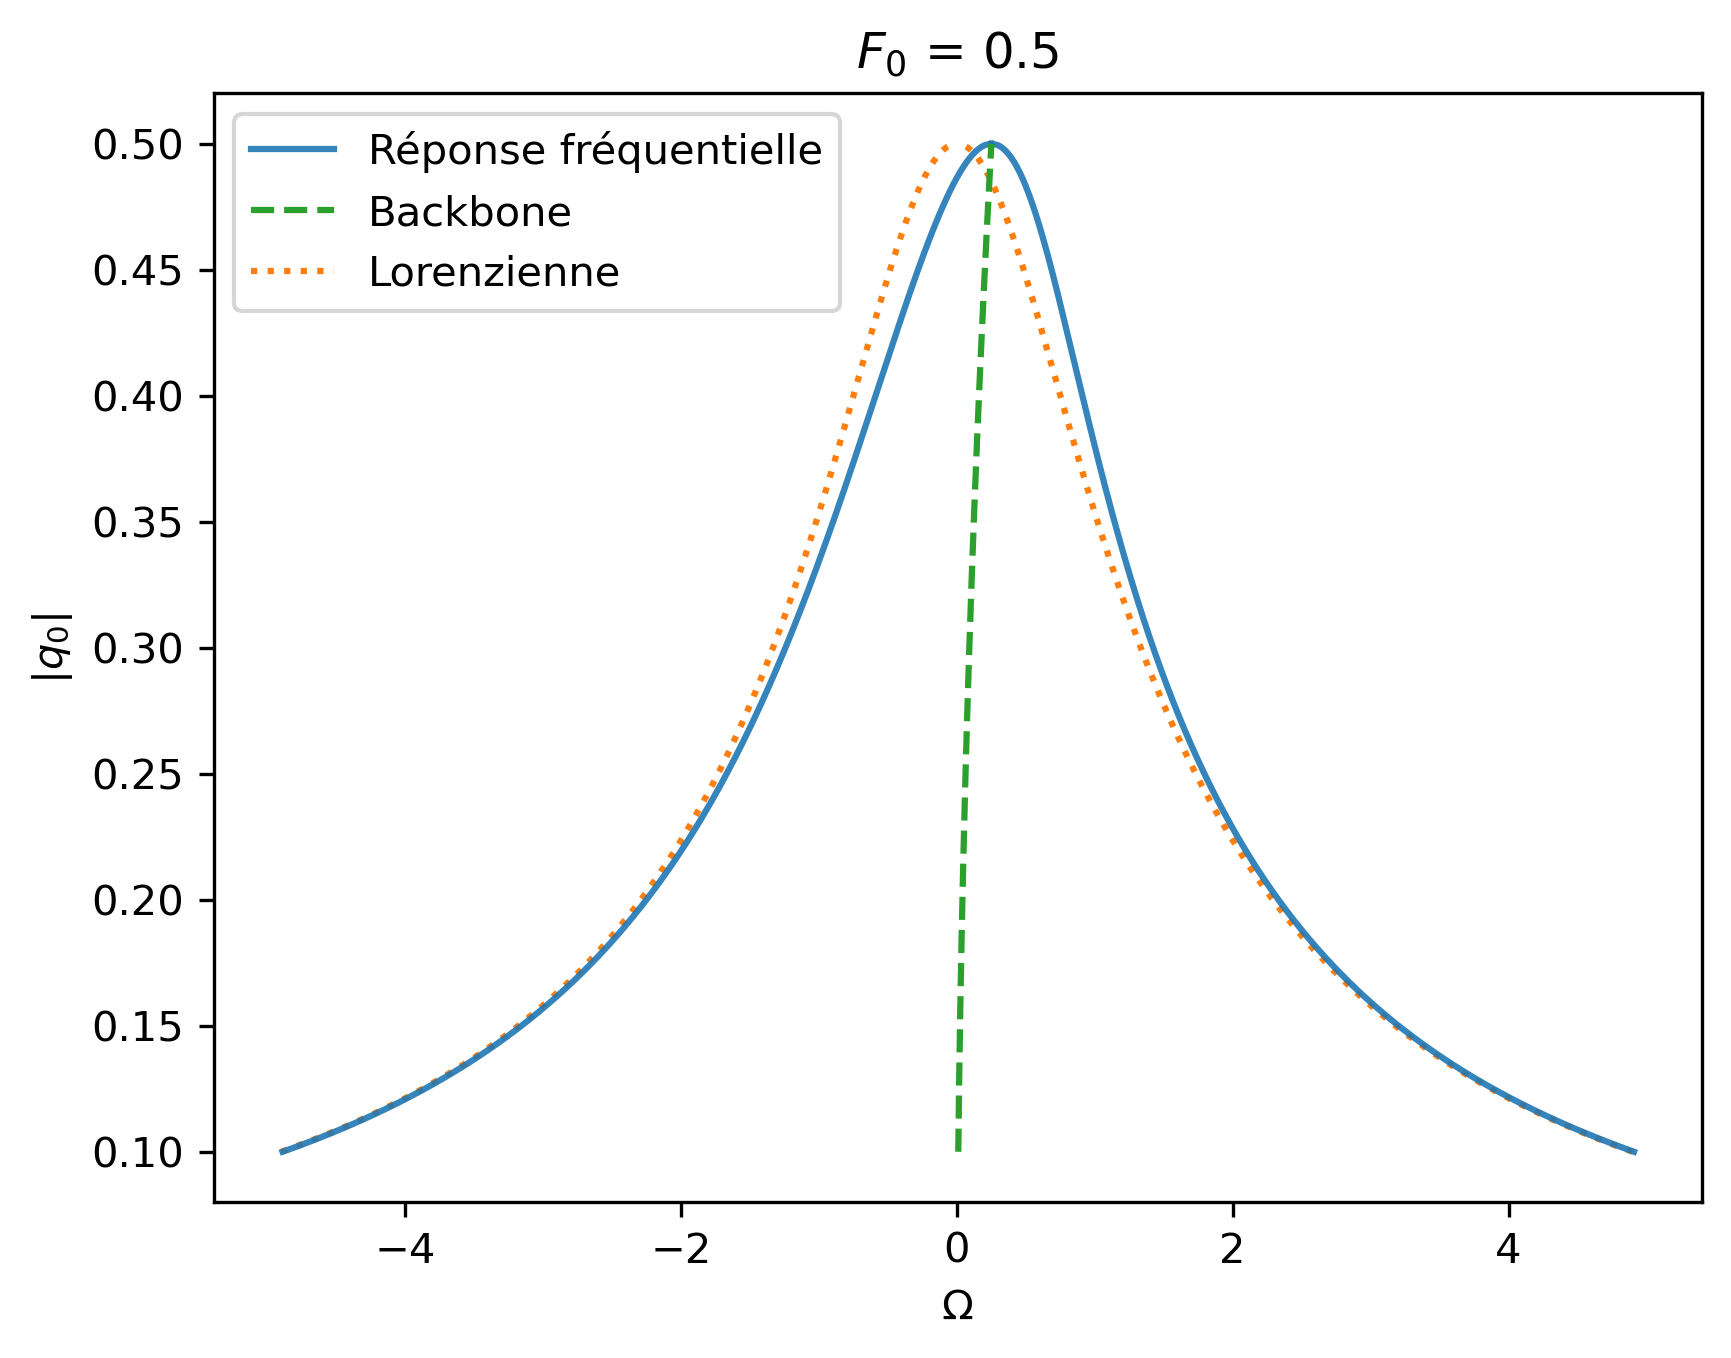
\includegraphics[width=\linewidth]{images/duffing/F0=0.5.png}%
    %   \phantomcaption
    % \end{subcaptionblock}
    % %\hfill
    % \begin{subcaptionblock}{.31\linewidth}
    %   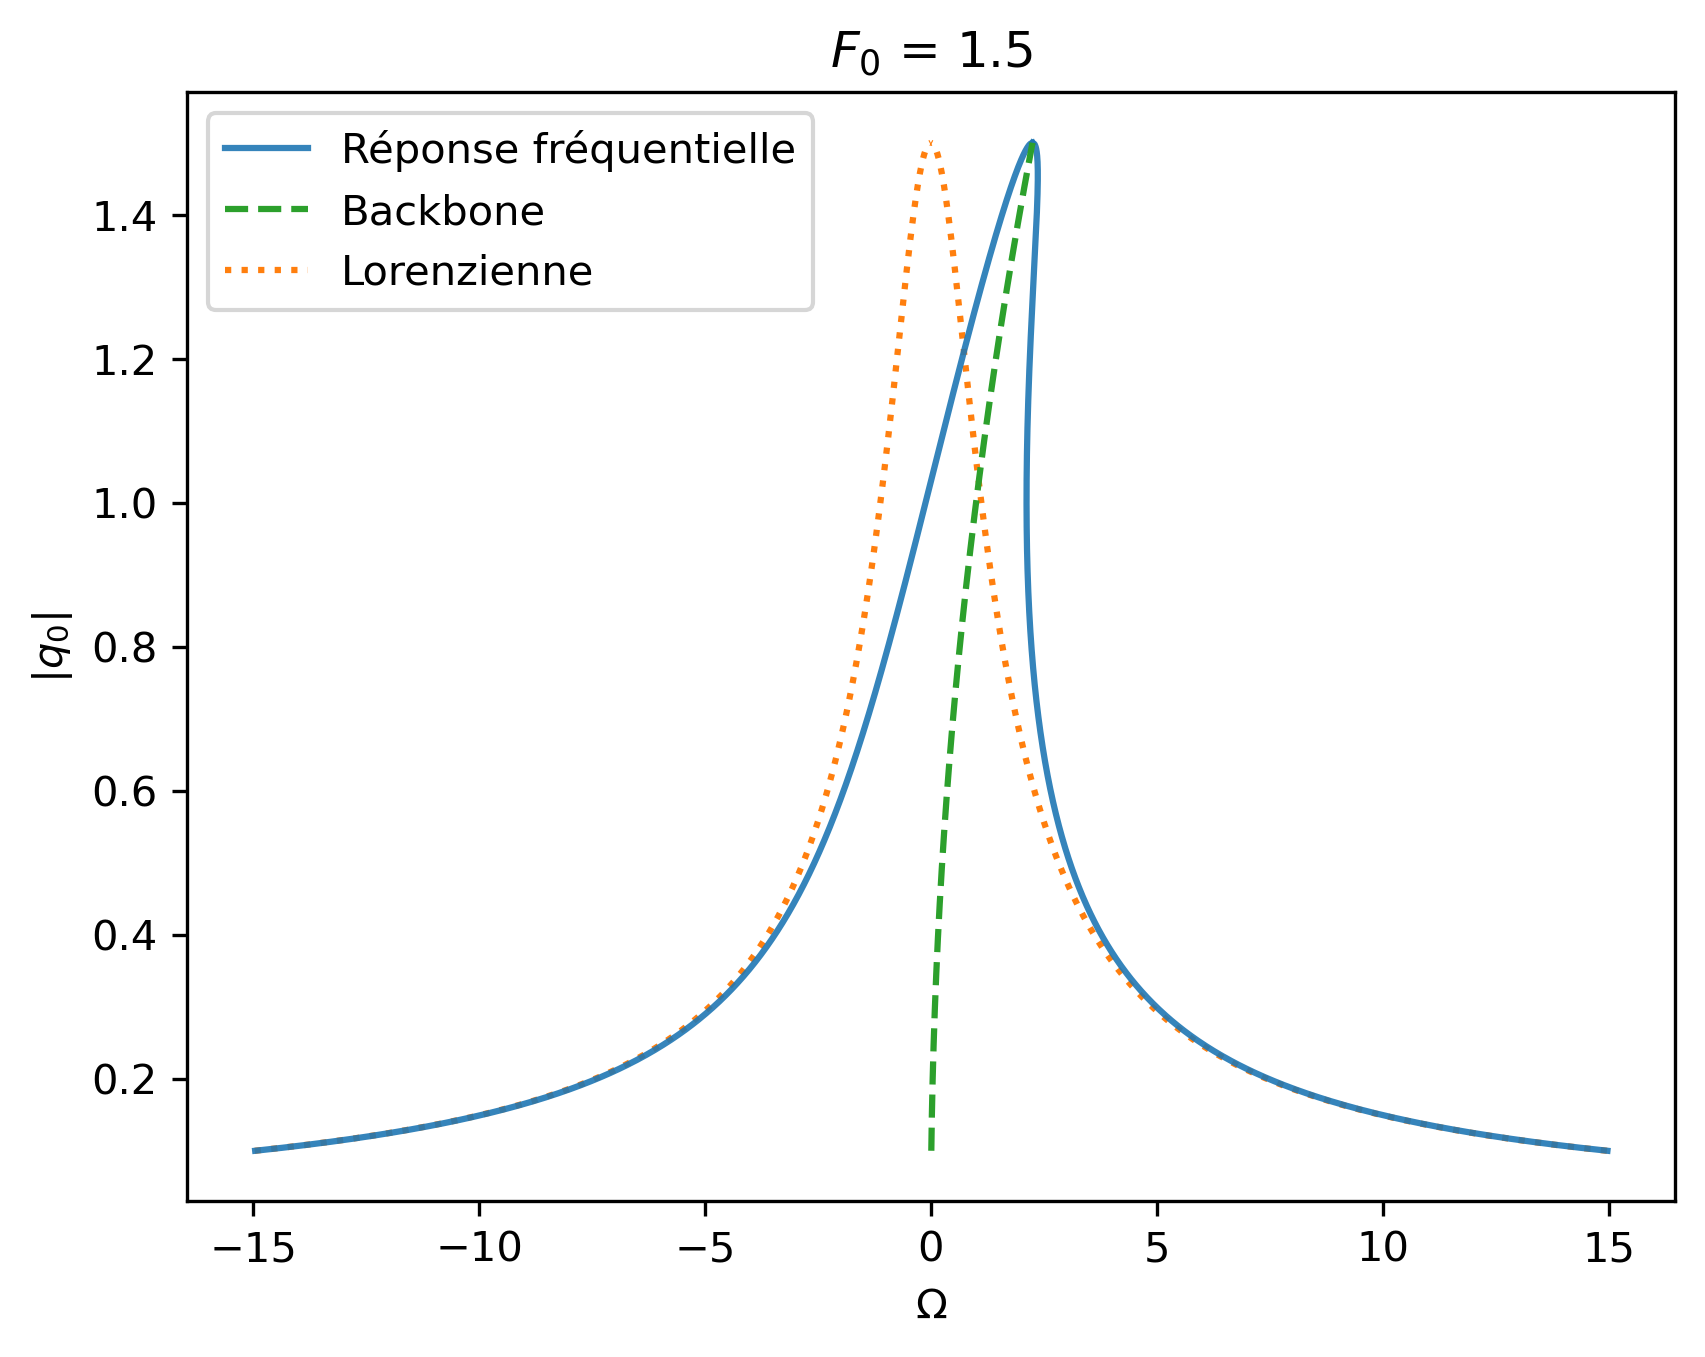
\includegraphics[width=\linewidth]{images/duffing/F0=1.5.png}%
    %   \phantomcaption
    % \end{subcaptionblock}
    % %\hfill
    % \begin{subcaptionblock}{.31\linewidth}
    %   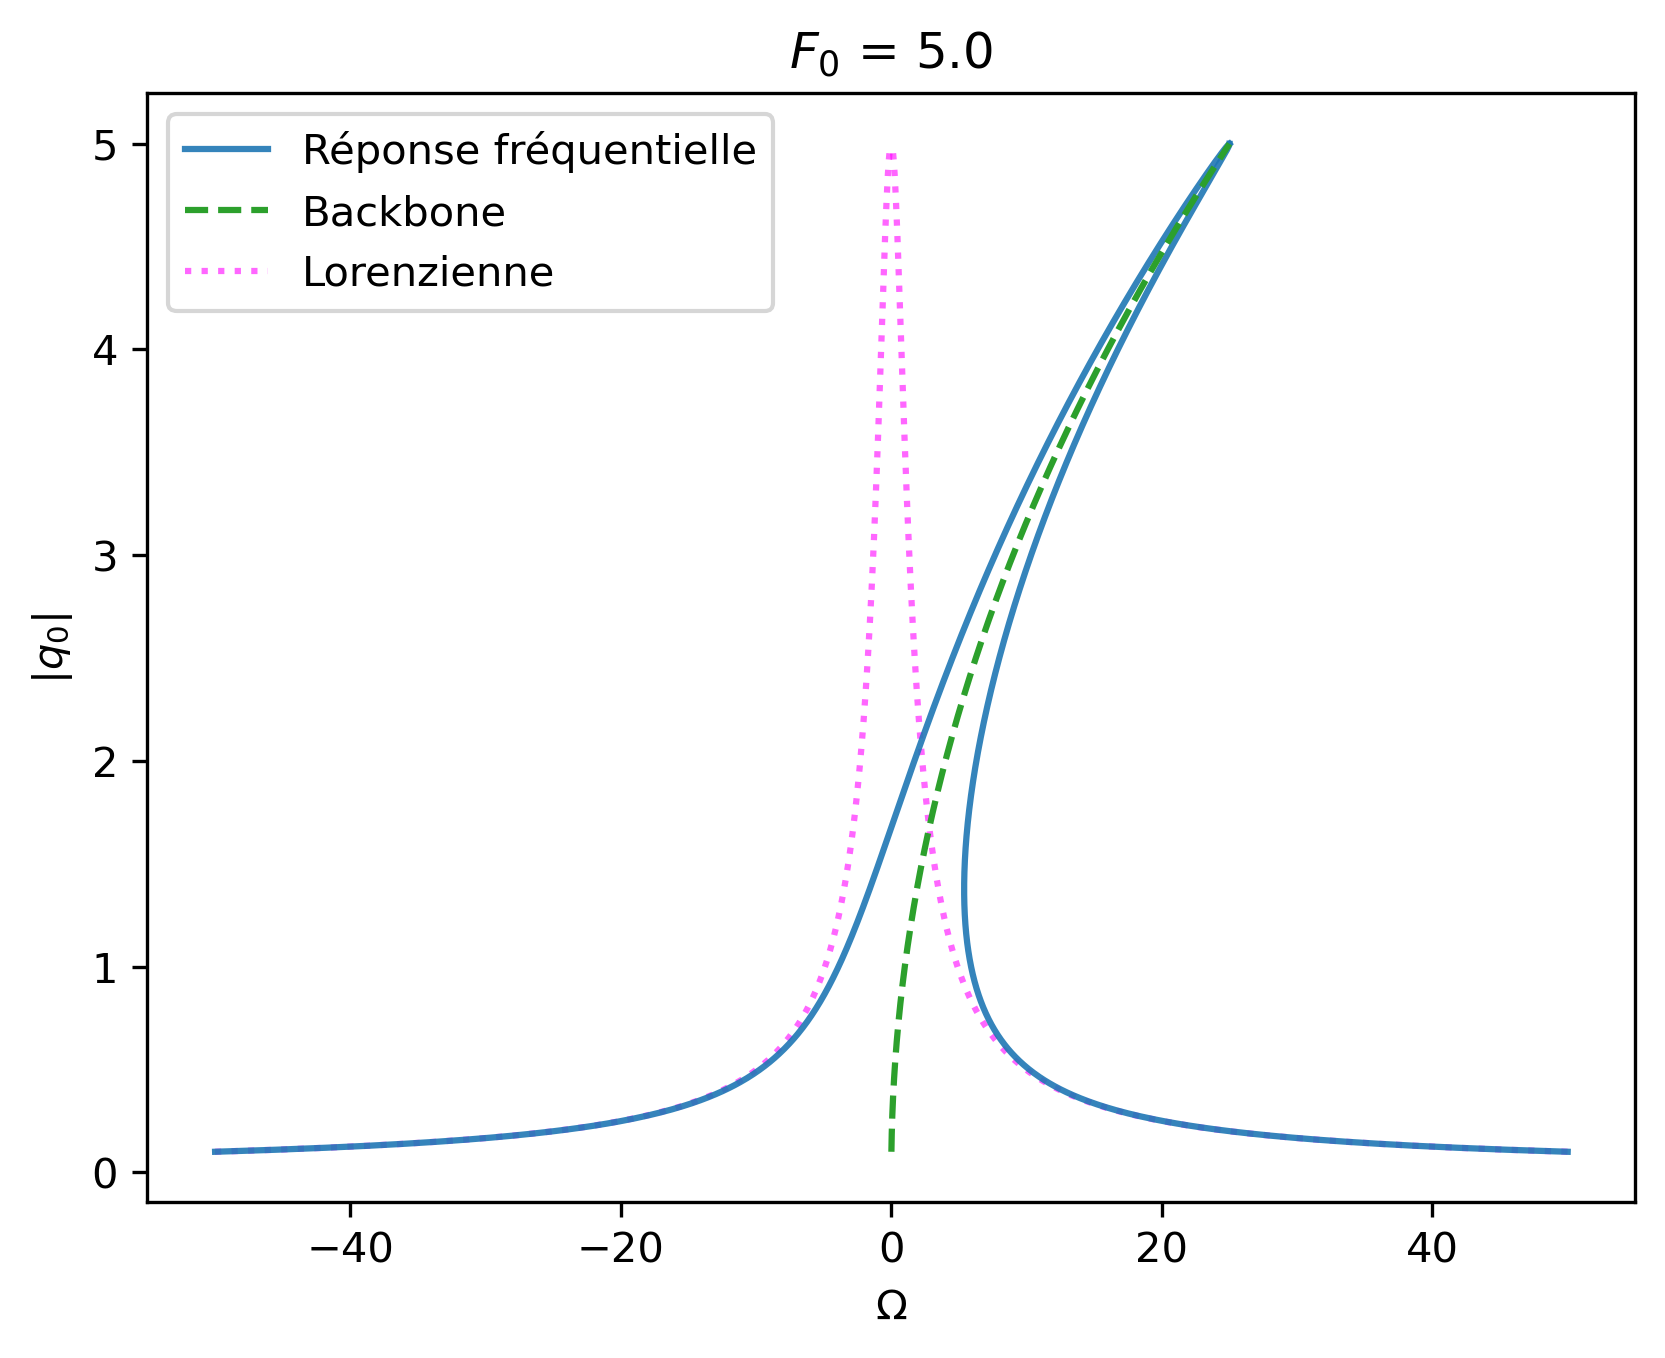
\includegraphics[width=\linewidth]{images/duffing/F0=5.0.png}
    %   \phantomcaption
    % \end{subcaptionblock}

    \begin{subfigure}[b]{0.32\textwidth}
         \centering
         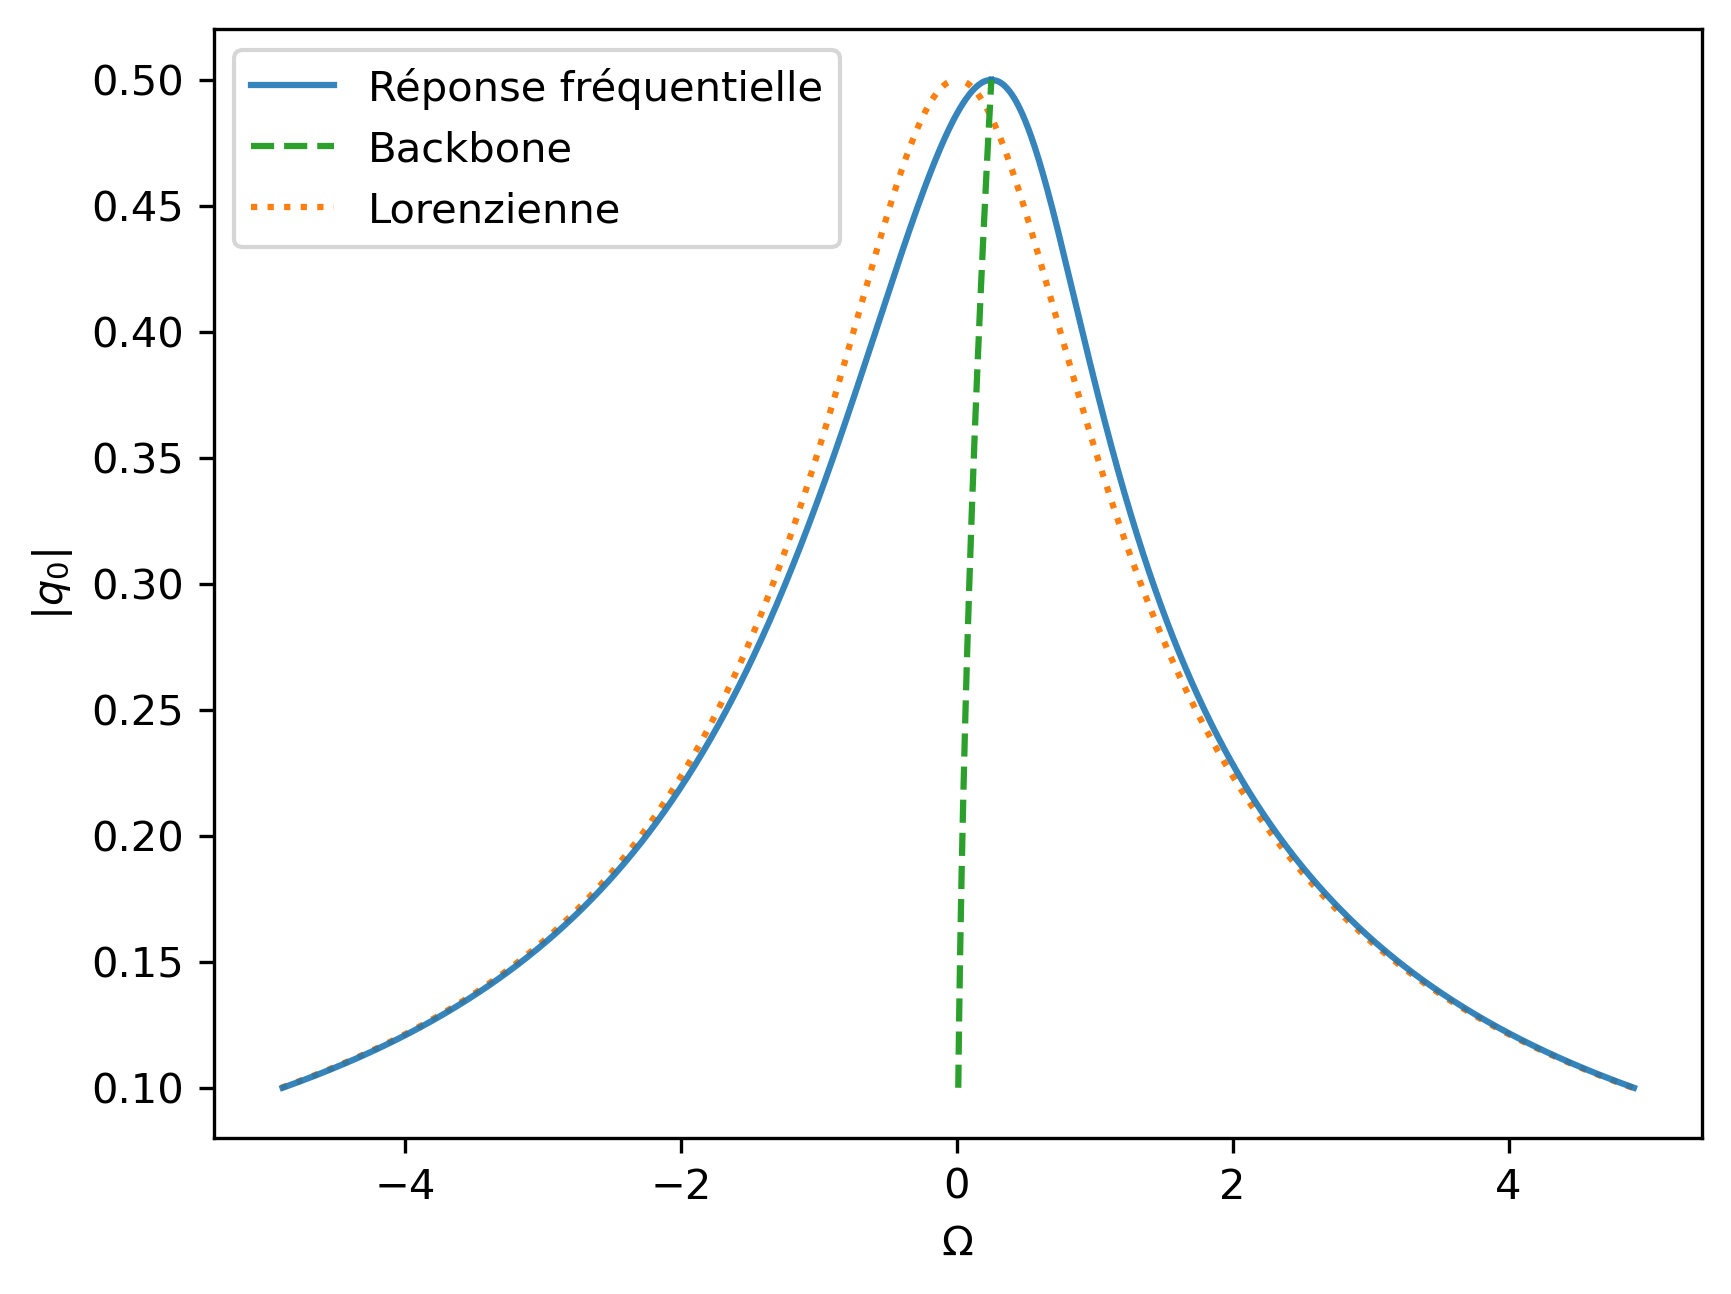
\includegraphics[width=\textwidth]{images/duffing/notitle_F0=0.5.png}
         \caption{}
         %\label{fig:comparison}
     \end{subfigure}  
     \hfill
     \begin{subfigure}[b]{0.315\textwidth}
         \centering
         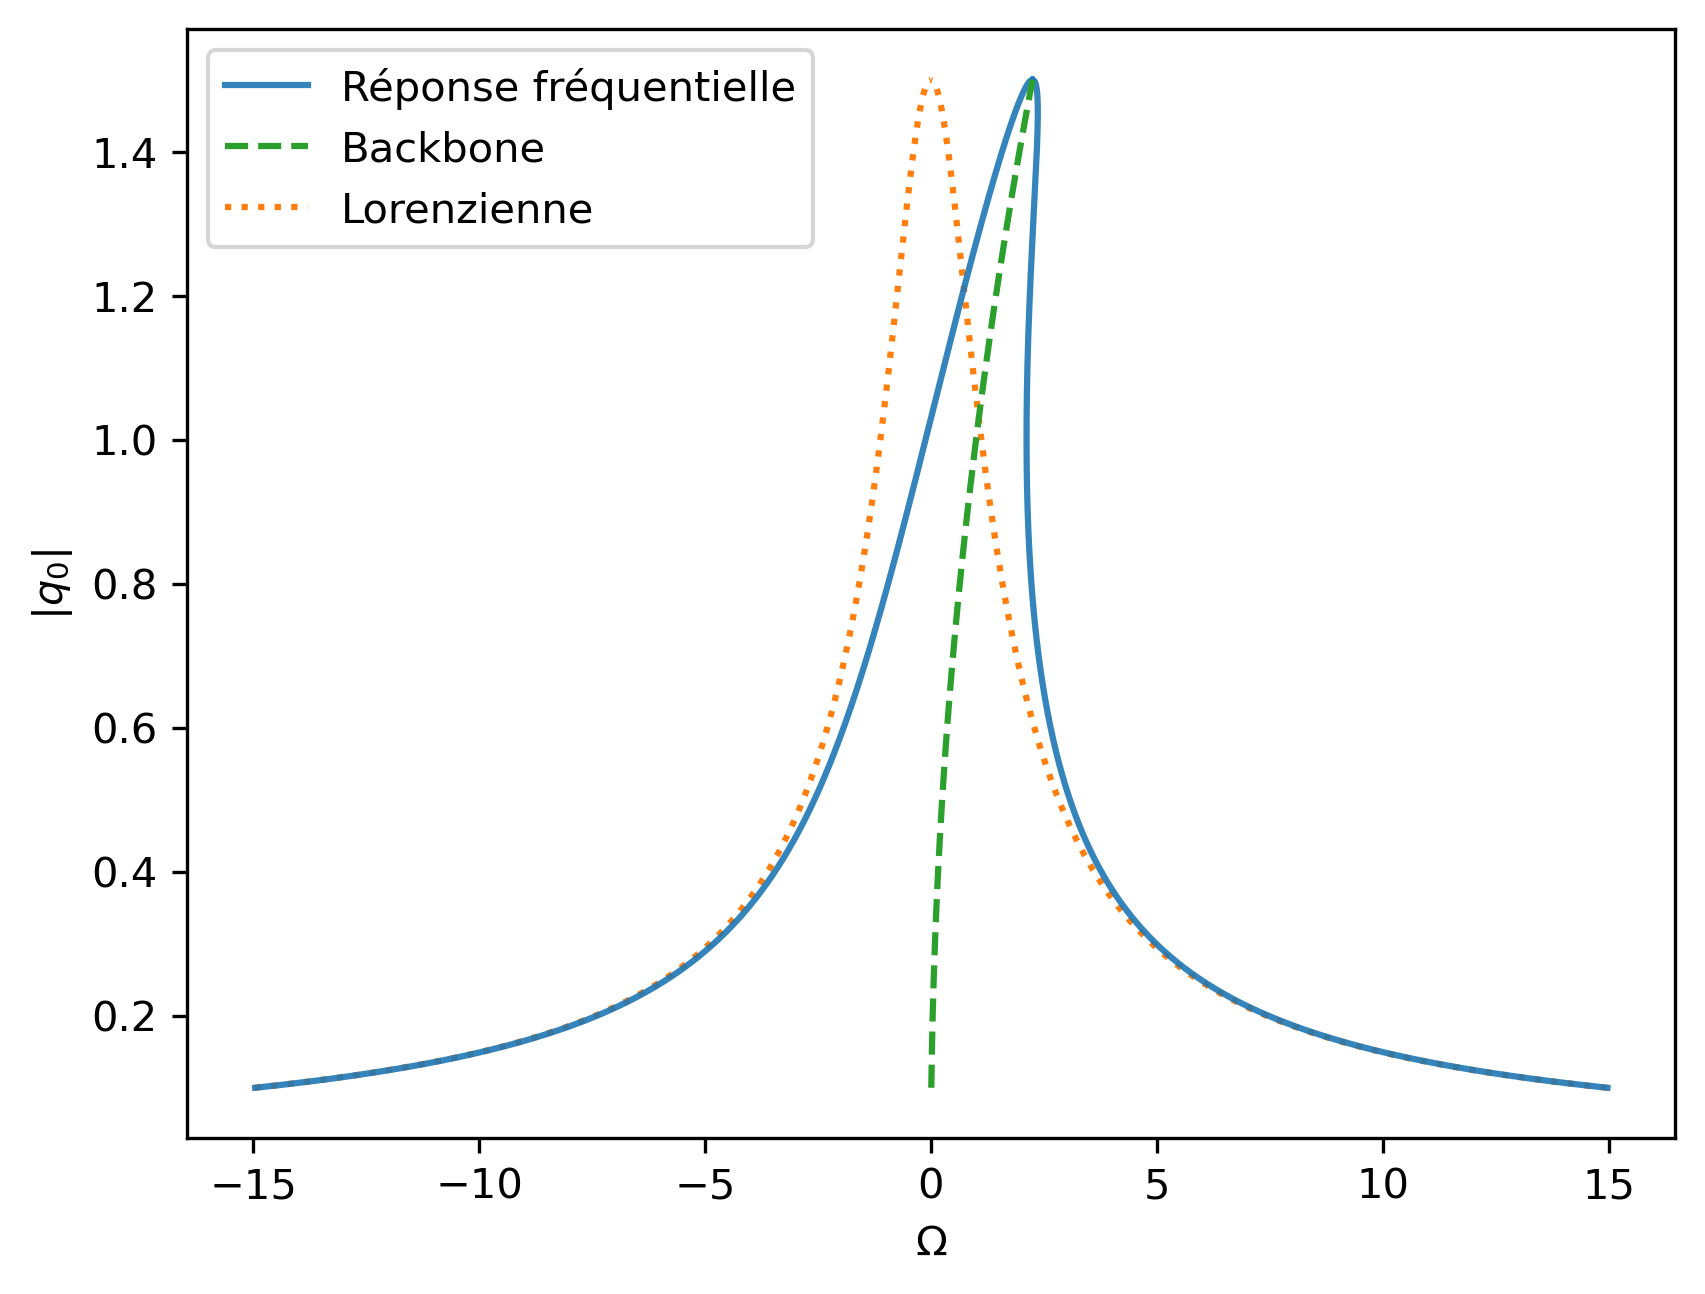
\includegraphics[width=\textwidth]{images/duffing/notitle_F0=1.5.png}
         \caption{}
         %\label{fig:comparison}
     \end{subfigure} 
     \hfill
     \begin{subfigure}[b]{0.31\textwidth}
         \centering
         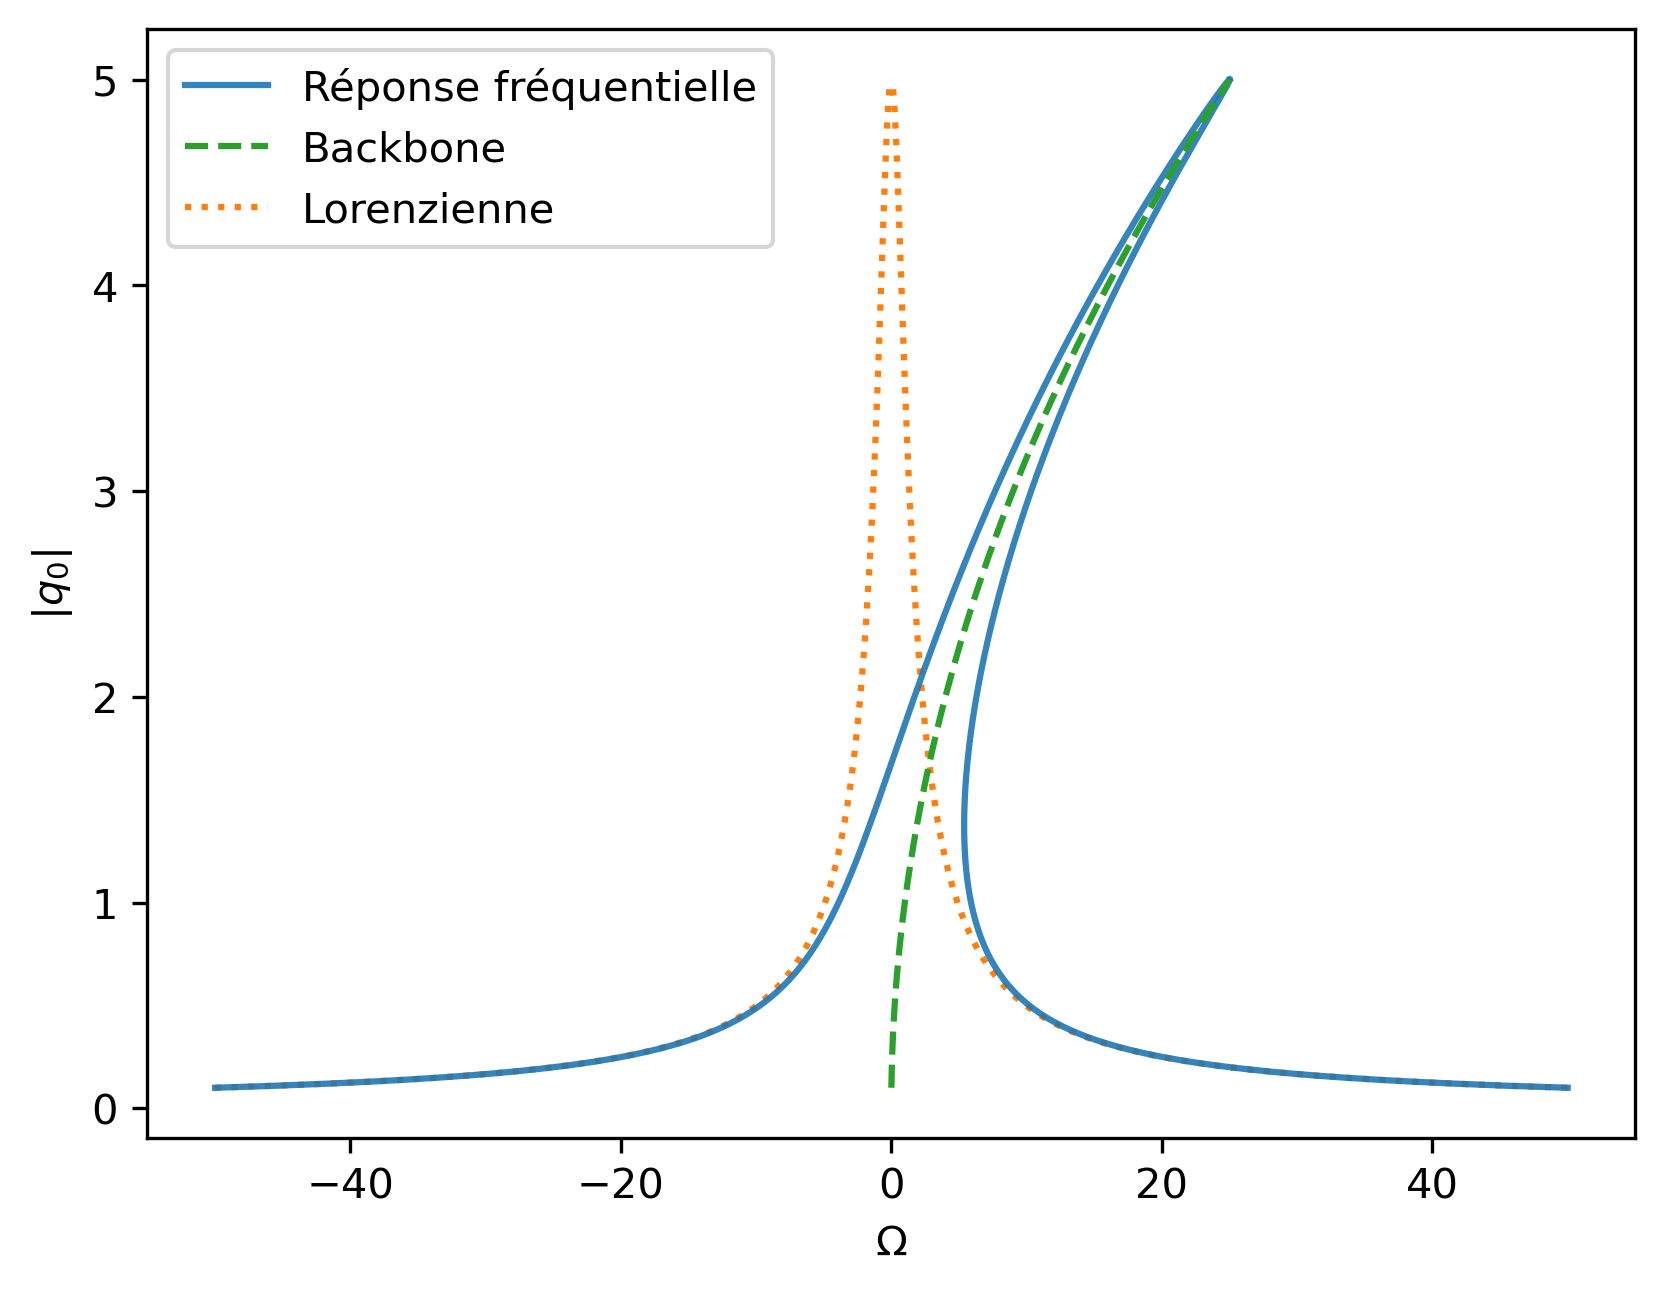
\includegraphics[width=\textwidth]{images/duffing/notitle_F0=5.0.png}
         \caption{}
         \label{fig:duff_freq_resp_3}
     \end{subfigure} 
    
    \caption{Réponses fréquentielles de Duffing obtenu à partir de \eqref{eq:duff_response} \textbf{(a)} $F_0=0.5$ \textbf{(b)} $F_0=1.5$ \textbf{(c)} $F_0=5.0$}
    \label{fig:duff_freq_resp_all}
\end{figure}

On cherche à déterminer la valeur de $F_{0, c}$. Pour alléger la notation, 
on introduit la variable $u = |q_0|$ et on réarrange \eqref{eq:duff_stationnaire} :
%
\begin{equation}
    u^2[(u^2 - \Omega)^2 + 1] = F_0^2
    \label{eq:duffing_stationnaire_in_u}
\end{equation}
%
Puis on prend la dérivée par rapport à $\Omega$.
%
\begin{equation}
    2u\frac{du}{d\Omega}(u^4 + \Omega^2 - 2\Omega u^2 + 1) + u^2(4u^3\frac{du}{d\Omega} + 2\Omega - 2u^2 - 4\Omega u\frac{du}{d\Omega}) = \frac{d}{d\Omega}F_0^2
\end{equation}
%
On remarque que $F_0$ et $\Omega$ dépendent tous les deux de $\omega$, qui est la vraie fréquence de forçage. Toutefois, pour dériver l'équation \eqref{eq:duff_stationnaire}, on a supposé $\omega \approx \omega_0$. Donc : 
%
\begin{equation*}
    \Omega \propto (\omega - \omega_0) \ll \omega
\end{equation*}
%
C'est-à-dire qu'en variant $\Omega$, la variation correspondante que subira $F_0$ sera très petite. Donc, on se permet de la considérer comme étant constante. En isolant $\frac{du}{d\Omega}$ on obtient :
%
\begin{equation}
    \frac{du}{d\Omega} = \frac{-\Omega u + u^3}{3u^4 + \Omega^2 - 4\Omega u^2 + 1}
\end{equation}
%
On peut d'abord déterminer l'amplitude maximum, qui est atteint lorsque $\frac{du}{d\Omega}=0$, en réinsérant cette condition dans \eqref{eq:duffing_stationnaire_in_u} on trouve :
%
\begin{equation*}
    |q_0|_{max} = F_0
\end{equation*}
%
La bistabilité apparait lorsque qu'il y a plusieurs points sur la courbe satisfaisant à $\frac{du}{d\Omega}=\infty$, nous donnant la condition :
%
\begin{equation}
    3u^4 + \Omega^2 - 4\Omega u^2 + 1 = 0
\end{equation}
%
Lorsque $F_0 = F_{0,c}$, il existe une unique solution en $u$. On peut donc résoudre pour $u^2$ en posant que le déterminant de l'équation quadratique s'annule. On obtient les conditions :
%
\begin{equation}
    \Omega = \pm \sqrt{3}
    \qquad
    u^2 = \frac{2\Omega}{3}
\end{equation}
%
Ce qui nous impose la solution unique $\Omega = \sqrt{3}$. En substituant ces valeurs dans \eqref{eq:duffing_stationnaire_in_u}, on trouve :
%
\begin{equation}
    F_{0,c} = \left(  \frac{8\sqrt{3}}{9}  \right)^{1/2} \approx 1.241
\end{equation}
%
Une observation finale intéressante. Étant donné que $F_0 \propto \epsilon^{3/2}f_0$, 
on voit que même dans un système ou le terme non-linéaire est très faible (où on ne s'attendrait pas à observer de non-linéarité). Il suffit d'augmenter l'amplitude de forçage $f_0$ 
pour faire ressortir un comportement non-linéaire (ici un état bistable). L'oscillateur harmonique pour modéliser les situations physiques n'est donc qu'une approximation valable à des amplitudes et à des forces relativement faibles.
